
Cyber-Physical Systems (CPS) are characterized by the strong interactions among cyber components and dynamic physical components.
CPS system examples include automotive and transportation systems, smart home, building and community,
smart battery and energy systems, surveillance systems, cyber-physical biochip, and wearable devices.
Due to the deeply complex intertwining among different components, CPS designs pose fundamental challenges in multiple aspects such as performance,
energy, security, reliability, fault tolerance and flexibility.
Innovative design techniques, algorithms and tools addressing the unique CPS challenges, such as the fast increase of system scale and complexity,
the close interactions with dynamic physical environment and human activities, the significant uncertainties in sensor readings,
the employment of distributed architectural platforms, and the tight real-time constraints, are highly desirable.

The IEEE TC-CCPS Newsletter, published twice a year, aims to report the recent advances on technologies, educations and opportunities and, consequently,
grow the research and education activities in this area.
This letter is affiliated with the Technical Committee on Cybernetics for Cyber Physical Systems under the IEEE Systems, Man, and Cybernetics Society.
TC-CCPS aims at promoting interdisciplinary research and education in the field of CPS.

This issue of the newsletter showcases the state-of-the-art developments covering several emerging areas:
machine monitoring, automobile, social cloud, energy, etc.
Professional articles are solicited from technical experts to provide an in-depth review of these areas.
These articles can be found in the section of ``Technical Articles''.
In the section of ``Technical Activities'', recent activities organized by the TC-CCPS, including workshops, special issues, etc., are summarized.
Finally, the Call for Contributions can be found at the end of this issue to solicit high-quality submissions.

I would like to express my great appreciation to all Associate Editors (Yier Jin, Rajiv Ranjan, Yiyu Shi, Bei Yu and Qi Zhu) for their dedicated effort and strong support in organizing this letter.
I wish to thank all authors who have contributed their professional articles to this issue.
Finally, please allow me to welcome all of you to the founding issue of the TC-CCPS Newsletter.
I hope that you will have an enjoyable moment when reading the letter!

\vspace{.2in}
\begin{figure}[h]
\begin{minipage}{.3\textwidth}
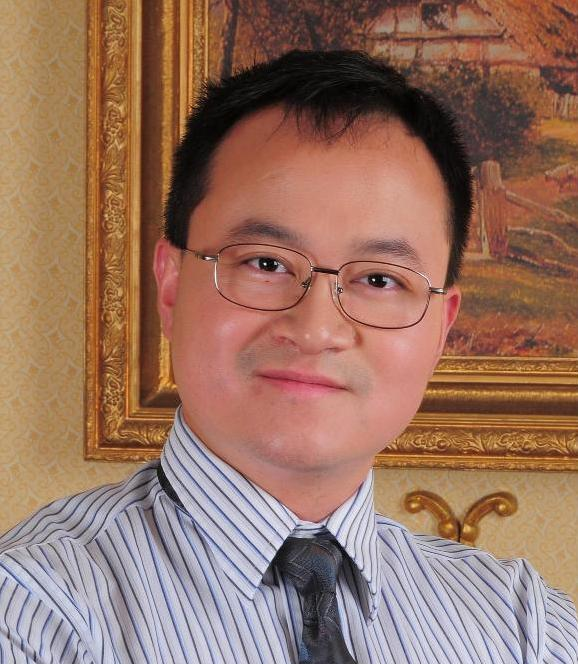
\includegraphics[width=2.5cm]{committee_xli.jpg}
\caption*{Xin Li \\ TC-CCPS Editor \\ Carnegie Mellon University}
\end{minipage}
\end{figure}

